% !TEX root = ../../../main.tex
% 来源：中学数学实验教材·第三册（高中数学）
% 章节：不等式和解不等式 / 解不等式
% 原始文件：3.tex，行 1991-2032
% 类型：tikz
% ---
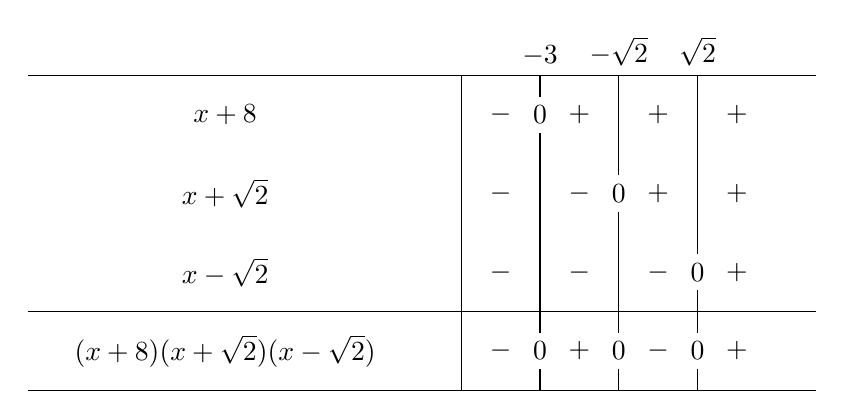
\begin{tikzpicture}[yscale=2]
\foreach \x in {0,.5,2}
{
    \draw (0,\x)--(10,\x);
}
\foreach \x/\xtext in {5.5/{},6.5/-3,7.5/-\sqrt{2},8.5/\sqrt{2}}
{
    \draw (\x,0)--(\x,2)node[above]{$\xtext$};
}

\node at (2.5,.25){$(x+8)(x+\sqrt{2})(x-\sqrt{2})$};
\foreach \x/\xtext in {6/-,7/+,8/-,9/+}
{
    \node at (\x,.25) {$\xtext$};
}

\node at (2.5,.75){$x-\sqrt{2}$};
\foreach \x/\xtext in {6/-,7/-,8/-,9/+}
{
    \node at (\x,.75) {$\xtext$};
}

\node at (2.5,1.25){$x+\sqrt{2}$};
\foreach \x/\xtext in {6/-,7/-,8/+,9/+}
{
    \node at (\x,1.25) {$\xtext$};
}

\node at (2.5,1.75){$x+8$};
\foreach \x/\xtext in {6/-,7/+,8/+,9/+}
{
    \node at (\x,1.75) {$\xtext$};
}


\node at (6.5,1.75)[fill=white] {0};
\node at (6.5,.25)[fill=white] {0};
\node at (7.5,.25)[fill=white] {0};
\node at (8.5,.25)[fill=white] {0};
\node at (8.5,.75)[fill=white] {0};
\node at (7.5,1.25)[fill=white] {0};
\end{tikzpicture}
